\newcommand{\duedatetime}{See Canvas for the due date}
% 16384_doc.cls lives in latex/ relative to this file; input@path lets
% \documentclass find it there without changing directory structure.
\makeatletter
\def\input@path{{latex/}}
\makeatother
\documentclass{16384_doc}

\newcommand{\assignmentname}{Assignment 6: Rigid Body Dynamics}
\graphicspath{{latex/}}

\ifdef{\writeup}{\printanswers}

\begin{document}
\maketitle
\tableofcontents

\section{Overview}
This assignment reinforces the following topics:
\begin{itemize}

\item Rigid Body Dynamics

\end{itemize}

\section{Background}

\subsection{Standard Form}

As a reminder, the standard form for writing equations of motion is as follows:

\begin{center}
    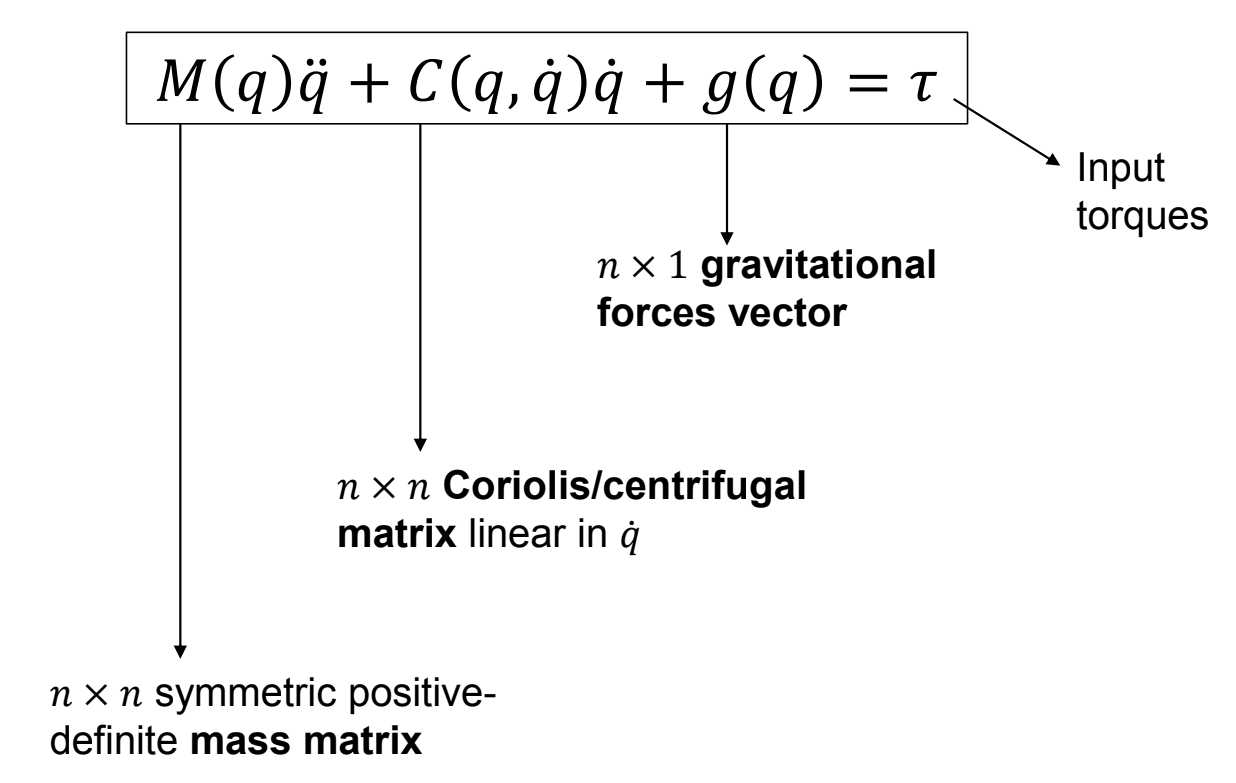
\includegraphics[width=\linewidth]{figures/standard_form.PNG}
\end{center}

\newpage

\writtenSection

% \section{In Class Question}
    
%     The following question will be done in class, as a part of a group. Your group's answer will still need to be turned in with the rest of your assignment, however unlike the rest of the work this is allowed to be done in groups.

% \begin{questions}
    
%     \titledquestion{Rigid Body Dynamics}
    
%     Please use the diagram of the arm below for the following questions:

%     \begin{center}
%     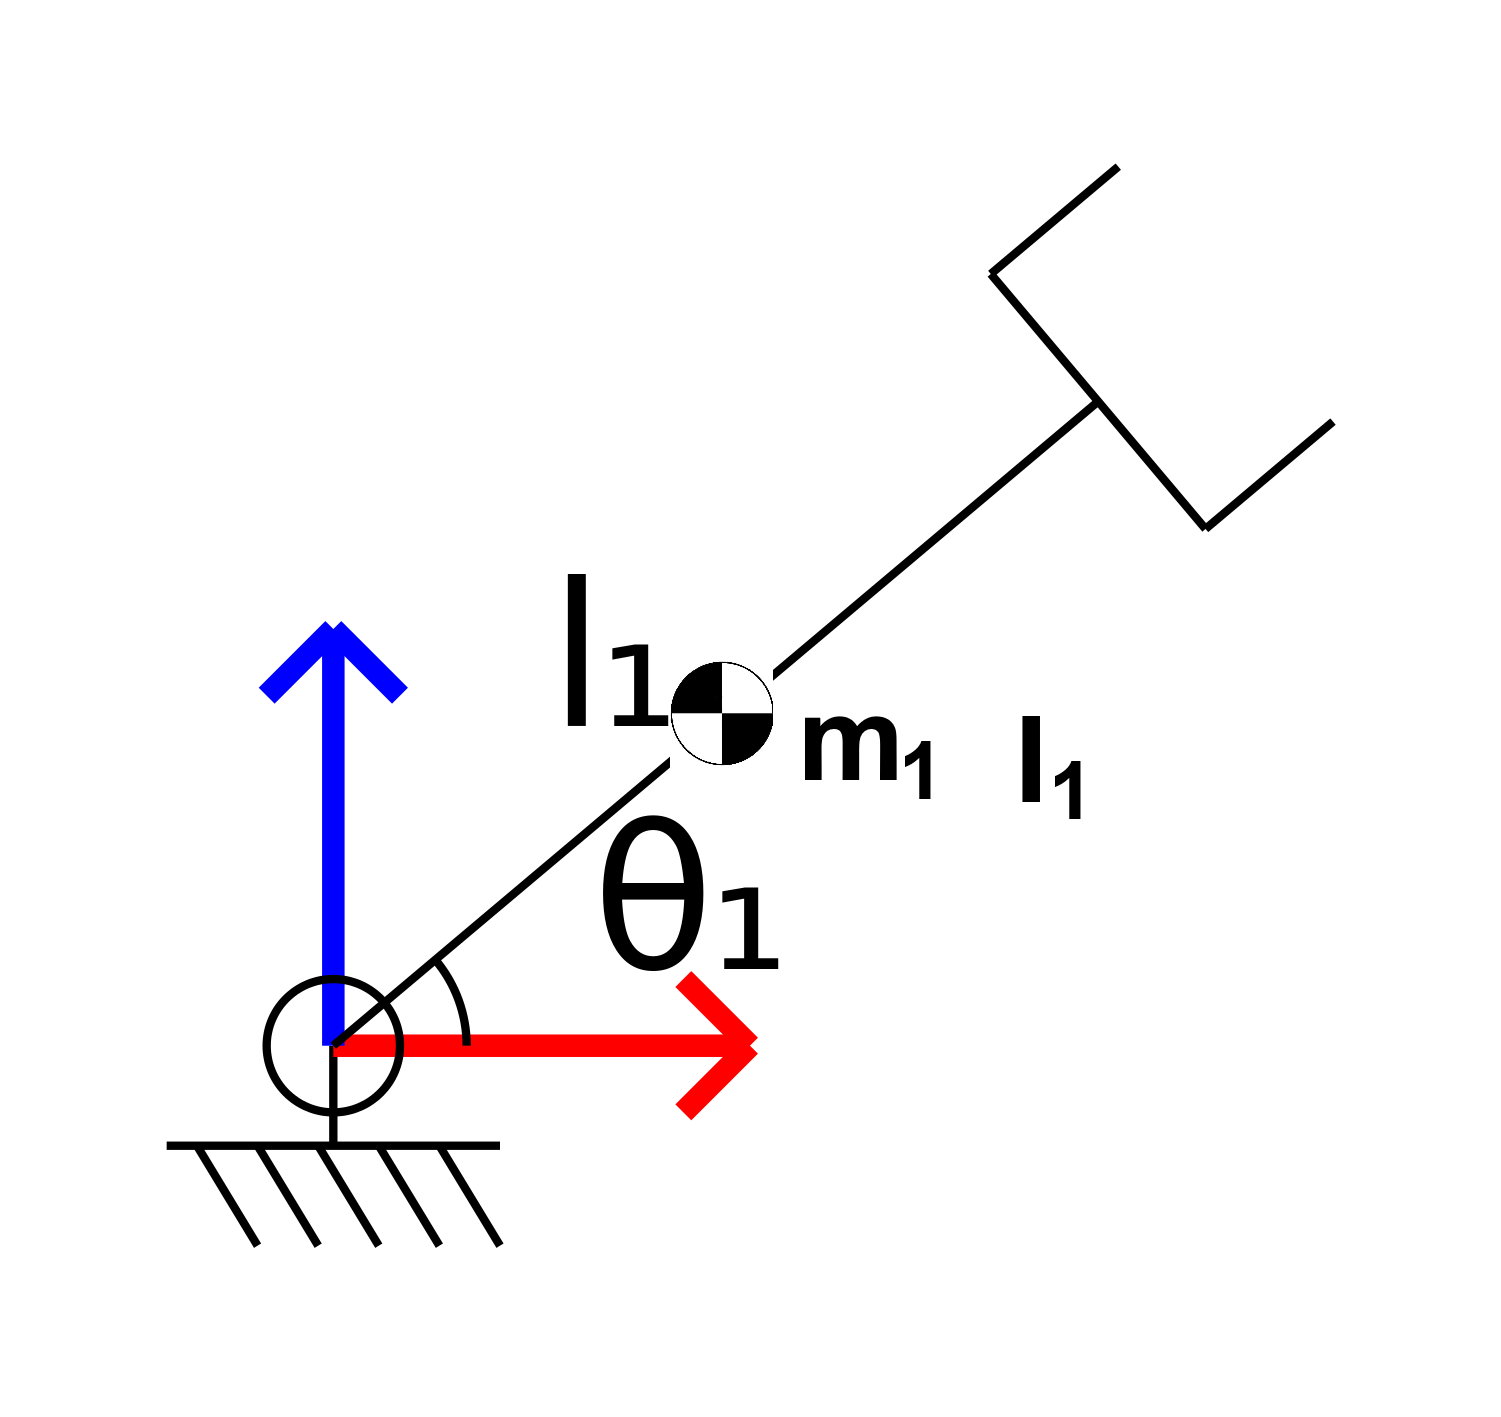
\includegraphics[width=0.33\linewidth]{figures/R_Robot_with_Inertia.png}
%     \end{center}
    
%     The arm has a link length of $l_1$ where the center of mass is located in the center of the link at $\frac{l_1}{2}$. The link's mass is $m_1$ and it has moment of inertia $I_1$. 

%     \begin{parts}
%         \part[5] Determine the Kinetic Energy for the R arm shown above.
        
%         \begin{tcolorbox}[height=11cm]
%          % TODO: ENTER YOUR ANSWER HERE
%         \end{tcolorbox}
        
%         \part[5] Determine the Potential Energy for the R arm shown above.
        
%         \begin{tcolorbox}[height=11.5cm]
%          % TODO: ENTER YOUR ANSWER HERE
%         \end{tcolorbox}
        
%         \part[5] Write the Lagrangian for the R arm shown above.
        
%         \begin{tcolorbox}[height=9.5cm]
%          % TODO: ENTER YOUR ANSWER HERE
%         \end{tcolorbox}
        
%         \part[5] Determine the Equations of Motion for the R arm shown above using the Lagrangian.
        
%         \begin{tcolorbox}[height=21.5cm]
%          % TODO: ENTER YOUR ANSWER HERE
%         \end{tcolorbox}
        
%         \part[5] Rewrite the equations of motion into standard form.
        
%         \begin{tcolorbox}[height=22cm]
%          % TODO: ENTER YOUR ANSWER HERE
%         \end{tcolorbox}
        
%     \end{parts}
    
% \end{questions}

% \section{Written Questions}
% For all of the following questions, please fully compute all answers and show
% your work for full credit, unless otherwise specified. Submit your answers in a
% PDF entitled \verb!writeup.pdf! in your handin directory.  All answers must be
% typed, but diagrams may be hand-drawn and scanned in.  However, they must be
% tidy and fully legible! Consider drawing them in a black or blue pen.  All units
% are in radians and meters, where appropriate.

\section{Written Section}

\begin{questions}
    
    \titledquestion{Rigid Body Dynamics}
    
    Please use the diagram of the arm below for the following questions:

    \begin{center}
    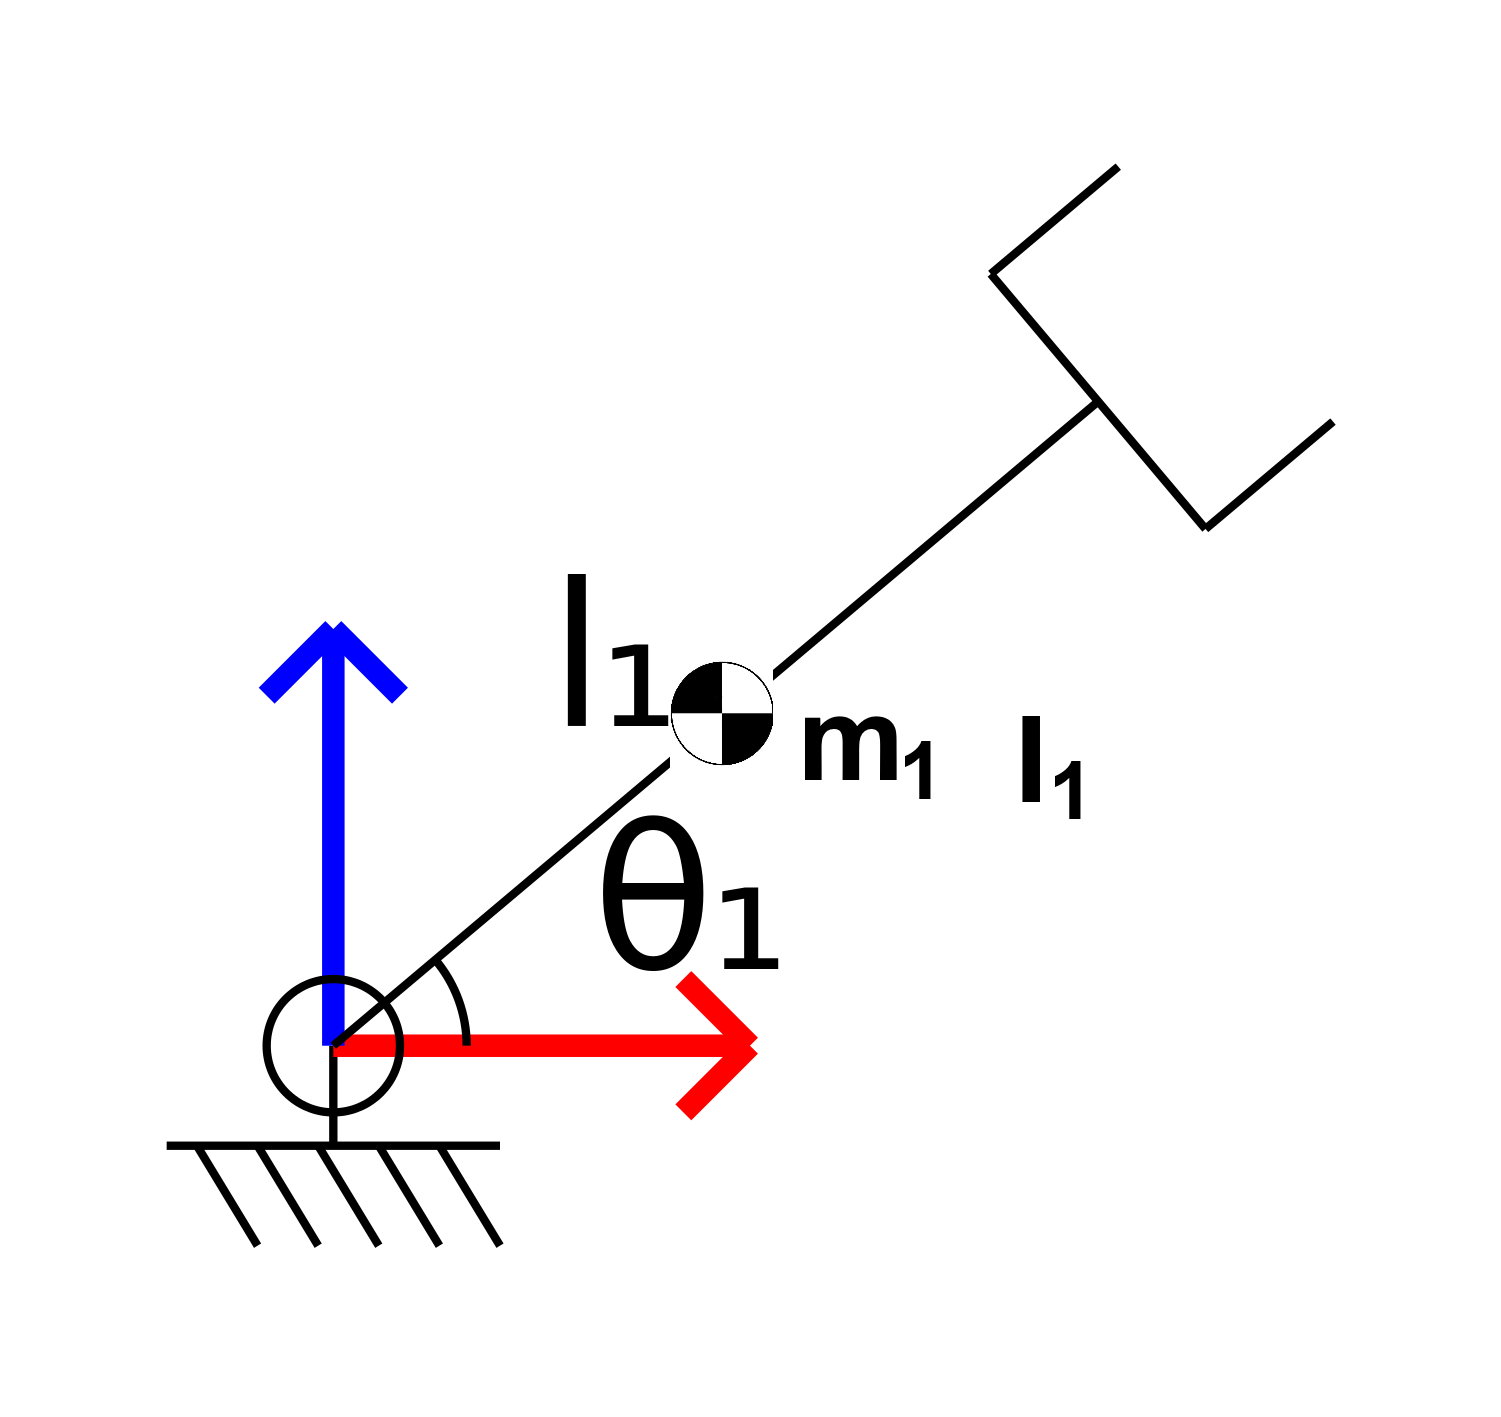
\includegraphics[width=0.33\linewidth]{figures/R_Robot_with_Inertia.png}
    \end{center}
    
    The arm has a link length of $l_1$ where the center of mass is located in the center of the link at $\frac{l_1}{2}$. The link's mass is $m_1$ and it has moment of inertia $I_1$. 

    \begin{parts}
        \part[5] Determine the Kinetic Energy for the R arm shown above.
        
        \begin{tcolorbox}[height=11cm]
         % TODO: ENTER YOUR ANSWER HERE
        \end{tcolorbox}
        
        \part[5] Determine the Potential Energy for the R arm shown above.
        
        \begin{tcolorbox}[height=11.5cm]
         % TODO: ENTER YOUR ANSWER HERE
        \end{tcolorbox}
        
        \part[5] Write the Lagrangian for the R arm shown above.
        
        \begin{tcolorbox}[height=9.5cm]
         % TODO: ENTER YOUR ANSWER HERE
        \end{tcolorbox}
        
        \part[5] Determine the Equations of Motion for the R arm shown above using the Lagrangian.
        
        \begin{tcolorbox}[height=21.5cm]
         % TODO: ENTER YOUR ANSWER HERE
        \end{tcolorbox}
        
        \part[5] Rewrite the equations of motion into standard form.
        
        \begin{tcolorbox}[height=22cm]
         % TODO: ENTER YOUR ANSWER HERE
        \end{tcolorbox}
        
    \end{parts}

    \titledquestion{RR robot}
    Consider the following robot

    \begin{center}
    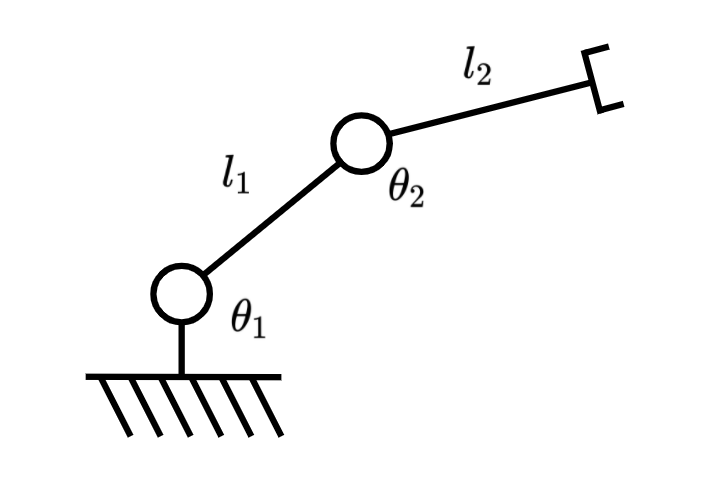
\includegraphics[scale=0.5]{figures/RR.png}
    \end{center}

    Given the above RR arm, each with a mass of $m_i$ located at $l_i/2$ and a moment of intertia of $I_i$ about their com 

    \newpage

    \begin{parts}
        \part[5] Determine the Kinetic Energy for the RR arm shown above.
        
        \begin{tcolorbox}[height=11cm]
         % TODO: ENTER YOUR ANSWER HERE
        \end{tcolorbox}
        
        \part[5] Determine the Potential Energy for the RR arm shown above.
        
        \begin{tcolorbox}[height=10cm]
         % TODO: ENTER YOUR ANSWER HERE
        \end{tcolorbox}
        
        \part[2] Write the Lagrangian for the RR arm shown above.
        
        \begin{tcolorbox}[height=10cm]
         % TODO: ENTER YOUR ANSWER HERE
        \end{tcolorbox}
        
        \part[10] Determine the Equations of Motion with respect to $\theta_1$ for the RR arm shown above using the Lagrangian.
        
        \begin{tcolorbox}[height=10cm]
         % TODO: ENTER YOUR ANSWER HERE
        \end{tcolorbox}
        
        \part[10] Determine the Equations of Motion with respect to $\theta_2$ for the RR arm shown above using the Lagrangian.
        
        \begin{tcolorbox}[height=10cm]
         % TODO: ENTER YOUR ANSWER HERE
        \end{tcolorbox}
        
        \part[5] Rewrite the equations of motion into standard form.
        
        \begin{tcolorbox}[height=10cm]
         % TODO: ENTER YOUR ANSWER HERE
        \end{tcolorbox}
        
    \end{parts}

    \titledquestion{3D Pendulum}
    Consider the following robot

    \begin{center}
    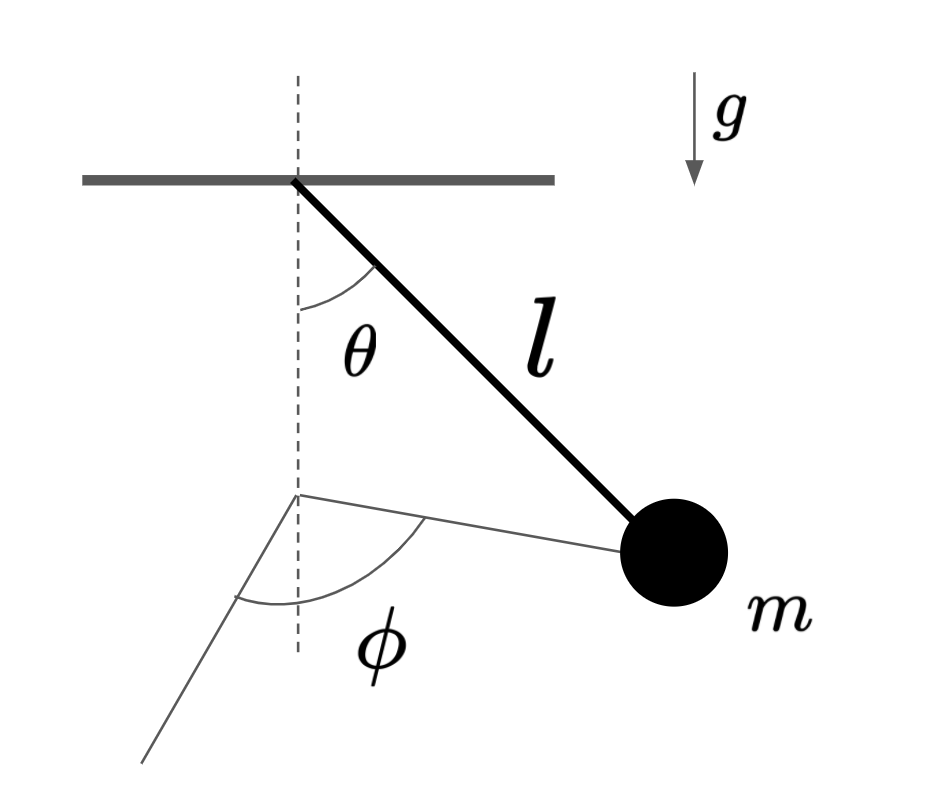
\includegraphics[scale=0.3]{figures/pendulum2.png}
    \end{center}

    Given a pendulum that can move anywhere in 3D space, with a fixed length l and a mass m, solve for its equations of motion. Hint: use spherical coordinates. 

    \newpage

    \begin{parts}
        \part[5] Determine the Kinetic Energy for 3D pendulum.
        
        \begin{tcolorbox}[height=11cm]
         % TODO: ENTER YOUR ANSWER HERE
        \end{tcolorbox}
        
        \part[5] Determine the Potential Energy for the 3D pendulum.
        
        \begin{tcolorbox}[height=10cm]
         % TODO: ENTER YOUR ANSWER HERE
        \end{tcolorbox}
        
        \part[2] Write the Lagrangian for the 3D pendulum.
        
        \begin{tcolorbox}[height=10cm]
         % TODO: ENTER YOUR ANSWER HERE
        \end{tcolorbox}
        
        \part[10] Determine the Equations of Motion with respect to $\theta$ for the 3D pendulum.
        
        \begin{tcolorbox}[height=10cm]
         % TODO: ENTER YOUR ANSWER HERE
        \end{tcolorbox}
        
        \newpage 
        \part[10] Determine the Equations of Motion with respect to $\phi$ for the 3D pendulum.
        
        \begin{tcolorbox}[height=10cm]
         % TODO: ENTER YOUR ANSWER HERE
        \end{tcolorbox}
        
        \part[5] If $\phi$ is kept constant, what do the equations above reduce to? What system that we've studied in class has similar EOMs?
        
        \begin{tcolorbox}[height=10cm]
         % TODO: ENTER YOUR ANSWER HERE
        \end{tcolorbox}
        
    \end{parts}
\end{questions}


\section{Code Questions}

There is no coding portion in this homework.

\begin{submissionChecklist}
		\item Create a PDF of your answers to the written questions with the name \verb!writeup.pdf!.
		\item Upload \verb!writeup.pdf! to Gradescope.
\end{submissionChecklist}

\end{document}
